\newcommand{\scaler}{0.5}
\newcommand{\soilwidth}{16cm*\scaler}
\newcommand{\soilheight}{20cm*\scaler}
\newcommand{\housewidth}{6cm*\scaler}
\newcommand{\side}{1cm*\scaler}
\newcommand{\ots}{0.2cm*\scaler}
\begin{center}


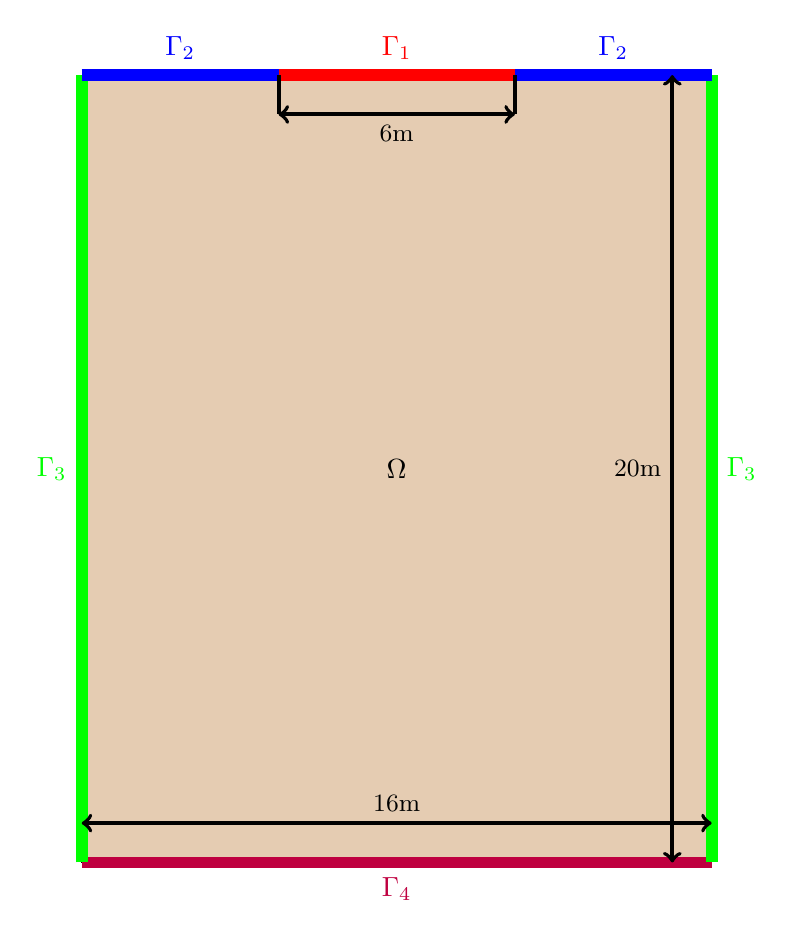
\begin{tikzpicture}
\draw [fill=brown!40!white] (0,0) rectangle node {$\Omega$} (\soilwidth,\soilheight);
  \coordinate (A1) at (0, 0);
  \coordinate (A2) at (\soilwidth, 0);

  \coordinate (B1) at (0, \soilheight);
  \coordinate (B2) at (\soilwidth/2-\housewidth/2, \soilheight);
  \coordinate (B3) at (\soilwidth/2+\housewidth/2, \soilheight);
  \coordinate (B4) at (\soilwidth, \soilheight);
  
  \coordinate (S1) at (\soilwidth - \side, 0);
  \coordinate (S2) at (\soilwidth - \side, \soilheight);
  
  \coordinate (S3) at (0, \side);
  \coordinate (S4) at (\soilwidth, \side);
  
  \coordinate (S5) at (\soilwidth/2-\housewidth/2, \soilheight - \side);
  \coordinate (S6) at (\soilwidth/2+\housewidth/2, \soilheight - \side);
  
  \draw [line width = 0.3cm*\scaler, color = purple] (A1) -- node [below] {$\Gamma_4$}(A2);
  \draw [line width = 0.3cm*\scaler, color = green] (A1) -- node [left] {$\Gamma_3$}(B1) (A2) -- node [right] {$\Gamma_3$}(B4);
  \draw [line width = 0.3cm*\scaler, color = blue] (B1) -- node [above] {$\Gamma_2$}(B2) (B3) -- node [above] {$\Gamma_2$}(B4);
  \draw [line width = 0.3cm*\scaler, color = red] (B2) -- node [above] {$\Gamma_1$} (B3);

\draw[arrows=<->,line width=0.1cm*\scaler] (S1) -- node [left] {\small{20m}} (S2);

\draw[arrows=<->,line width=0.1cm*\scaler] (S3) -- node [above] {\small{16m}} (S4);
\draw[line width = 0.1cm*\scaler] (B2) -- (S5) (B3) -- (S6);
\draw[arrows=<->,line width=0.1cm*\scaler] (S5) -- node [below] {\small{6m}} (S6);

\end{tikzpicture}
\end{center}